\newpage
\newpage
%%%%%%%%%%%%%%%%%%%%%%%%%%%%%%%%%%%%%%%%%%%%%
%%% Chapter 1:  Radiation in IR
%%%%%%%%%%%%%%%%%%%%%%%%%%%%%%%%%%%%%%%%%%%%%
\chapter{Introduction}

\section{Interventional Radiology}
Interventional radiology (IR) is a subspecialty of radiology that utilizes fluoroscopy to perform diagnostic and therapeutic procedures through minimally invasive techniques \cite{8}. Fluoroscopy involves the use of X-rays and an image detection system to visualize internal structures and interventional tools in real-time \cite{11}. 
\begin{figure}[H]
 \centering
  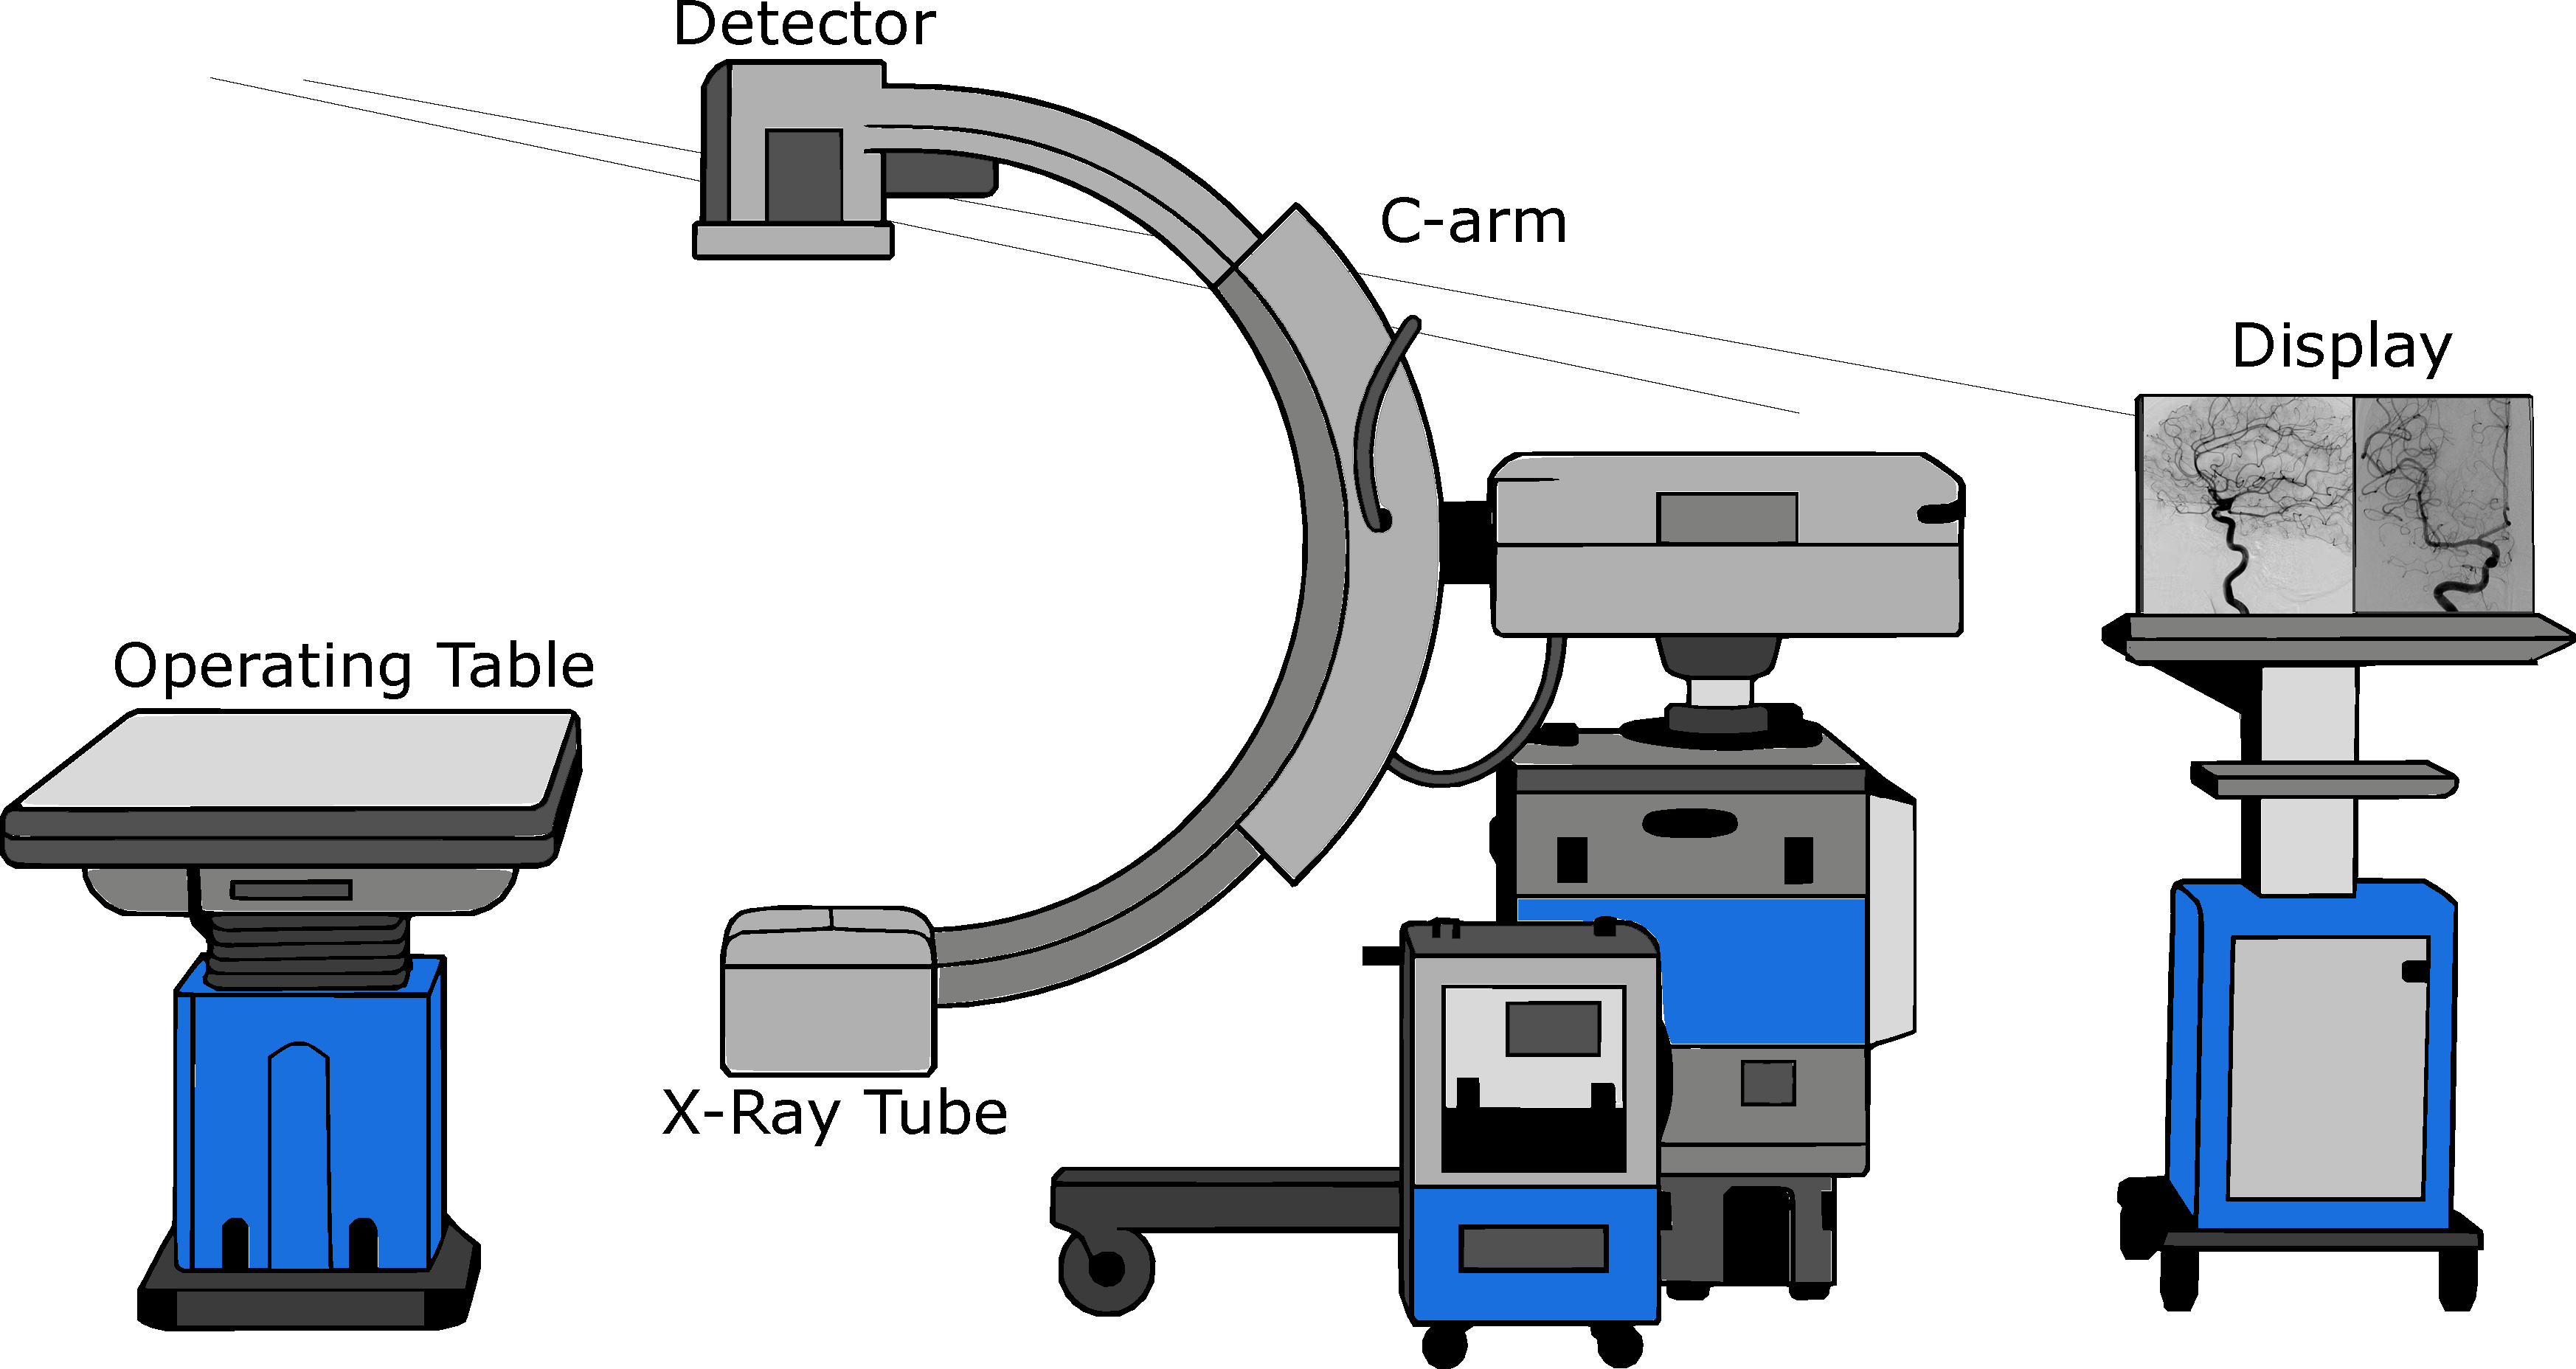
\includegraphics[width=\linewidth]{images/interventional radiology setup.pdf}
 \caption[Interventional Radiology Setup]{Interventional Radiology Setup. The C-arm is positioned in a posteroanterior projection (standard clinical practice) directing the most intense backscatter towards the floor, protecting above-knee radiosensitive organs~\cite{26}. The images shown on the display monitor were reproduced from Refs.~\cite{111,112}.}

 \label{fig:interventional_radiology_setup}
\end{figure}
The conventional IR equipment configuration is illustrated in Fig.~\ref{fig:interventional_radiology_setup}. The X-rays are produced in an X-ray tube by converting the kinetic energy of electrons into electromagnetic radiation. It consists of two electrodes enclosed in a vacuum-sealed glass envelope. The cathode serves as the electron source, while the anode acts as the positive target. When heated by an electric current, the cathode emits electrons via thermionic emission. The number of electrons produced depends on the current passing through the filament. A high potential difference applied between the cathode and the anode accelerates the electrons toward the anode. The total incident energy delivered to the anode is proportional to both the voltage and the current\cite{5,6}.

The X-rays transmitted through the patient strike the image detection system, mounted opposing the X-ray tube on a C-arm gantry. In the standard configuration, the X-ray tube is positioned beneath the patient table and the detector above, capitalising on the anisotropic distribution of scattered radiation to minimise occupational exposure~\cite{21,22}. The detector converts incident X-rays into visible light, which is optically transmitted to a camera system and displayed on a monitor to guide interventions in real-time. For continuous fluoroscopy, a steady tube current is supplied and images are acquired at 30 frames per second to maintain the perception of smooth motion~\cite{16}. Table~\ref{tab:ir_parameters} outlines common technical parameters used in IR procedures \cite{20}.
% Small vertical space after surrounding text
\vspace{1em}

% Manual table title, numbered and added to LoT
\refstepcounter{table}
\label{tab:ir_parameters}
\noindent\textbf{Table~\thetable.} Representative ranges of technical parameters used in IR procedures. Adapted from Ref.~\cite{20}.%
\addcontentsline{lot}{table}{\protect\numberline{\thetable}Representative ranges of technical parameters used in IR procedures.}

% Small space between title and table
\vspace{0.1em}

\begin{table}[H]
  \centering
  \begin{tabular}{>{\raggedright\arraybackslash}p{0.08\textwidth}
                  >{\centering\arraybackslash}p{0.08\textwidth}
                  >{\centering\arraybackslash}p{0.08\textwidth}
                  >{\centering\arraybackslash}p{0.11\textwidth}
                  >{\centering\arraybackslash}p{0.11\textwidth}
                  >{\centering\arraybackslash}p{0.11\textwidth}
                  >{\centering\arraybackslash}p{0.11\textwidth}
                  >{\centering\arraybackslash}p{0.09\textwidth}}

    \toprule
\scriptsize \textbf{Parame\-ter} & \scriptsize \textbf{Peak high voltage} & \scriptsize \textbf{Tube current} & \scriptsize \textbf{Inherent Al filtration} & \scriptsize \textbf{Cu filtration} & \scriptsize \textbf{Pulse duration} & \scriptsize \textbf{Pulse frequency} & \scriptsize \textbf{Scatter Energy} \\

    \midrule
    \scriptsize \textbf{Range}
& \scriptsize 60–120 kV
& \scriptsize 5–1000 mA
& \scriptsize 4.5 mm
& \scriptsize 0.2–0.9 mm
& \scriptsize 1–20 ms
& \scriptsize 1–30 Hz
& \scriptsize 20–100 keV \\
    \bottomrule
  \end{tabular}
\end{table}

 \section{Photon Interaction with Matter}
 \label{sec:Photon Interaction with Matter}
X-rays interact with matter through four physical mechanisms: the photoelectric effect, Compton scattering, Rayleigh dispersion and pair production. The latter two are not relevant in IR~\cite{14}. Therefore, only the photoelectric effect and Compton scattering are considered in detail. Both processes are shown schematically in Fig.~\ref{fig:interaction}.
\subsection{Photoelectric Effect}
The photoelectric effect occurs when an incident photon transfers all of its energy to a bound electron within an atom, resulting in the ejection of the electron from its orbital. This process preferentially involves inner-shell electrons due to their greater electron density. The incident photon energy ($E_0$) is expended to overcome the binding energy of the electron ($E_b$), and any remaining energy is converted into the kinetic energy of the ejected photoelectron ($E_{\text{pe}}$), expressed as~\cite{5,6}:
\begin{equation}
E_{\text{pe}} = E_0 - E_b,\ \text{unit: } [\mathrm{keV}]
\label{eq:photoeletric}
\end{equation}
\indent
The vacancy is filled by an outer electron, with the release of a characteristic X-ray or an Auger electron. When these emissions are reabsorbed within the detector, the total deposited energy equals $E_0$, recorded as the photopeak. As the emissions are monoenergetic, the photopeak would be a Dirac delta. However, and as shown in Fig.~\ref{fig:interaction} (a), the peak has a finite width, set by the energy resolution of the detector and is a property of the instrument~\cite{14}.

The probability of photoelectric interaction is predominant at lower energies ($<$50 keV). It is also dependent on atomic number, increasing with higher-$Z$ materials, which provides contrast in X-ray imaging. As a result, lower-energy X-ray beams produce higher contrast but also increase photon absorption in the patient, leading to a higher dose. In interventional planning, beam quality is therefore optimised to balance image quality and patient dose, as higher photon energies reduce patient absorption but increase the contribution of Compton scattering, leading to greater noise and poorer contrast~\cite{6}.
\begin{figure}[H]
  \centering
  \input{figures/Interaction_with_matter}
  \caption[Photon interactions in IR]{Schematic representation of the photoelectric effect \textbf{(a)} and Compton scattering \textbf{(b)}, and the resulting energy spectrum.}

  \label{fig:interaction}
\end{figure}


\subsection{Compton Scattering}
\label{sec:compton_scattering}
Compton scattering is an inelastic interaction in which an incident photon interacts with a free outer-shell electron, transferring part of its energy. As a result, the electron is ejected as a recoil (Compton) electron. In accordance with the conservation of energy and momentum, the photon is deflected at an angle $\theta$, dependent on the energy transferred. The energy of the scattered photon $E_c$ is described as~\cite{6}:
\begin{equation}
E_c = \frac{E_0}{1 + \frac{E_0}{511} (1 - \cos\theta)},\ \text{unit: } [\mathrm{keV}] \label{eq:compton}
\end{equation}

 Within the detector, all scattering angles are permitted, from $0^\circ$ to $180^\circ$. This creates a Compton continuum, bounded by the two extremes. The maximum energy transfer to the electron occurs at $\theta = 180^\circ$, the Compton Edge (CE). At the same angle, a photon scattered in the surrounding material may enter the detector and be absorbed, forming the backscatter peak shown in Fig.~\ref{fig:interaction} (b)~\cite{14}.

 At photon energies typical of diagnostic radiology, the scattered photon retains most of the initial energy and remains sufficiently energetic to penetrate tissue. Within this energy range, Compton scattering predominates over the photoelectric effect in materials such as soft tissue, water and air. The interaction probability is proportional to the physical density of the material, but it is independent of the atomic number due to the uniform electron density across soft tissues~\cite{5,6}.

\section{Dosimetry Fundamentals}

\subsection{Physical Quantities}
\subsubsection{\emph{KERMA}}
When a beam of indirectly ionizing radiation, such as X-rays, interacts with matter, it transfers energy to charged particles within the medium. The total energy transferred ($\varepsilon_{tr}$) within a volume, $V$, is defined as \cite{12}:
\begin{equation}
\varepsilon_{tr} = (R_{in})_u - (R_{out})_u^{\text{nonr}} + \sum Q,\ \text{unit: } [\mathrm{J}]
\label{eq:energy_transferred}
\end{equation}
\noindent where \((R_{\text{in}})_u\) and \((R_{\text{out}})_u\) are the radiant energies of uncharged particles entering and leaving the volume, respectively, excluding secondary radiative emissions. \(\sum Q\) represents changes in rest mass energy within \(V\).

The dosimetric quantity \emph{KERMA} (Kinetic Energy Released in MAtter) quantifies the initial kinetic energy transferred to char\-ged particles, per unit mass, regardless of where and how that energy is spent \cite{6,12}:
\begin{equation}
KERMA = \frac{d\varepsilon_{tr}}{dm},\ \text{unit: } \left[\frac{\mathrm{J}}{\mathrm{kg}}\right] \text{ or } [\mathrm{Gy}]
\label{eq:kerma}
\end{equation}
\subsubsection{Absorbed Dose}
Absorbed dose ($D$) incorporates all subsequent energy deposition mechanisms such as radiative losses, e.g. \emph{Bremsstrahlung}. The total deposited energy (\( \varepsilon \)) includes the energy balance defined in Eq. \ref{eq:energy_transferred}, along with all contributions from charged particles, per unit mass at a point of interest. $D$ is used to quantify the effects of radiation and is expressed as \cite{11,12}:
\begin{equation}
D = \frac{d\varepsilon}{dm},\ \text{unit: } [\mathrm{Gy}]
\label{eq:absorbed_dose}
\end{equation}

\subsubsection{Exposure}
Exposure ($X$) is the earliest defined dosimetric quantity and applies to photon interactions in air. It measures the amount of electric charge, \(dQ\), produced by ionization in a given mass of dry air \cite{12}:
\begin{equation}
X = \frac{dQ}{dm},\ \text{unit: } \left[\frac{\mathrm{C}}{\mathrm{kg}}\right]
\label{eq:exposure}
\end{equation}

Exposure is directly related to the collision component of \emph{KERMA}, (\(K_{col}\)). \(K_{col}\) represents the fraction of energy transferred that is deposited through ionization and excitation, excluding radiative losses. In fact, a connection between $X$ and \(K_{\text{col}}\) can be established through the quantity \(\overline{W}_{\text{air}}\), defined as the mean energy required to produce an ion pair in dry air (\(\overline{W}_{\text{air}} = 33.97~\mathrm{J/C}\)):
\begin{equation}
K_{\text{col, air}} = \overline{W}_{\text{air}} \cdot X = 33.97 \cdot X,\ \text{unit: } [\mathrm{Gy}]
\label{eq:kcair_exposure}
\end{equation}
\noindent
In practice, \(K_{\text{col, air}}\) is commonly referred to as \emph{air KERMA} and is used to describe the output of an X-ray tube, as it can be measured directly in free air \cite{11}.

\subsection{Protection Quantities}
Radiation effects on humans vary due to differences in bio\-logical response and are classified as either stochastic or deterministic. Deterministic effects (Fig.~\ref{fig:effects}~(a)), inclu\-ding development of cataracts or skin erythema, have a threshold dose and increase in severity with higher exposure.  Stochastic outcomes (Fig.~\ref{fig:effects}~(b)), such as cancer, occur statistically, with the probability increasing with dose but without a threshold. To reflect these probabilistic biological responses, additional weighting factors for radiation type and tissue radiosensitivity must be considered. Thus, two protection-related quantities, equivalent dose ($H$) and effective dose~($E$), are derived from absorbed dose~\cite{13,14}.
\begin{figure}[H]
  \centering
  \tikzset{every picture/.style={line width=0.75pt}}

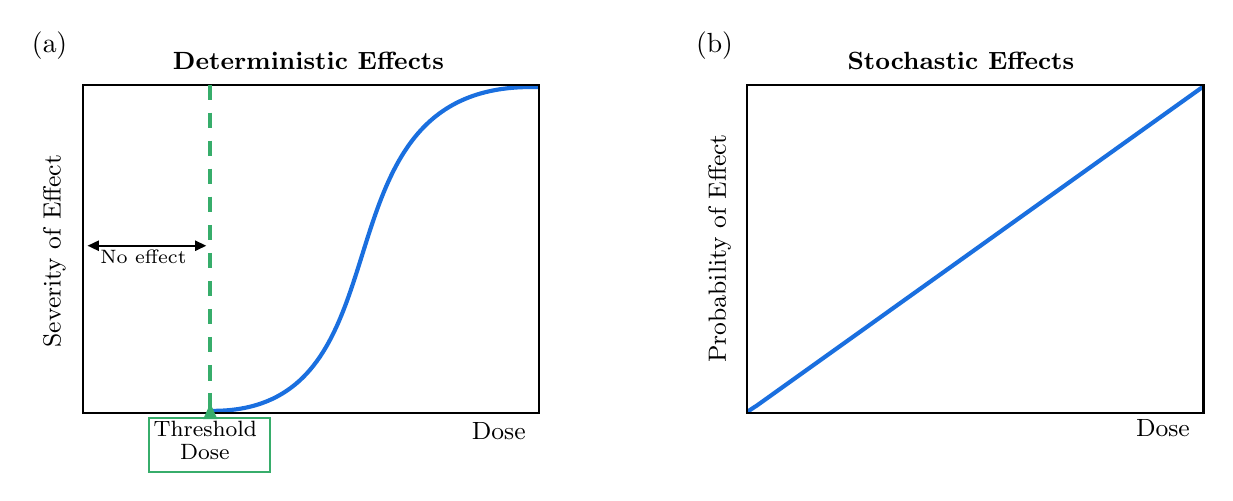
\begin{tikzpicture}[x=0.75pt,y=0.75pt,yscale=-1,xscale=1]

%Straight Lines [id:da7730700763729692] 
\draw [color={rgb, 255:red, 26; green, 111; blue, 223}  ,draw opacity=1 ][line width=1.5]    (599.76,48.96) -- (385.01,202.42) -- (380.42,205.43) ;
%Curve Lines [id:da8629624283311327] 
\draw [color={rgb, 255:red, 26; green, 111; blue, 223}  ,draw opacity=1 ][line width=1.5]    (121.47,205.11) .. controls (198.34,206.12) and (184.08,114.95) .. (221.47,71.53) .. controls (233.7,57.34) and (251.44,48.25) .. (279.69,49.16) ;
%Shape: Rectangle [id:dp07258514804006644] 
\draw  [line width=0.75]  (60,48) -- (280,48) -- (280,206) -- (60,206) -- cycle ;
%Straight Lines [id:da09166760913517435] 
\draw [color={rgb, 255:red, 55; green, 173; blue, 107}  ,draw opacity=1 ][line width=1.5]  [dash pattern={on 5.63pt off 4.5pt}]  (121.38,47.92) -- (121.38,206.32) ;
%Straight Lines [id:da3468358858445303] 
\draw    (65.4,125.56) -- (116.52,125.56) ;
\draw [shift={(119.52,125.56)}, rotate = 180] [fill={rgb, 255:red, 0; green, 0; blue, 0 }  ][line width=0.08]  [draw opacity=0] (5.36,-2.57) -- (0,0) -- (5.36,2.57) -- cycle    ;
\draw [shift={(62.4,125.56)}, rotate = 0] [fill={rgb, 255:red, 0; green, 0; blue, 0 }  ][line width=0.08]  [draw opacity=0] (5.36,-2.57) -- (0,0) -- (5.36,2.57) -- cycle    ;
%Shape: Rectangle [id:dp4467912586395093] 
\draw  [color={rgb, 255:red, 55; green, 173; blue, 107}  ,draw opacity=1 ] (91.8,208.57) -- (150.3,208.57) -- (150.3,234.63) -- (91.8,234.63) -- cycle ;
%Shape: Triangle [id:dp7577642747879886] 
\draw  [color={rgb, 255:red, 55; green, 173; blue, 107}  ,draw opacity=1 ][fill={rgb, 255:red, 55; green, 173; blue, 107}  ,fill opacity=1 ] (121.5,202.71) -- (124.14,208.56) -- (118.85,208.56) -- cycle ;
%Shape: Rectangle [id:dp10920079476550804] 
\draw  [line width=0.75]  (380,48) -- (600,48) -- (600,206) -- (380,206) -- cycle ;

% Text Node
\draw (102,31) node [anchor=north west][inner sep=0.75pt]  [font=\small] [align=left] {\textbf{Deterministic Effects}};
% Text Node
\draw (67,126) node [anchor=north west][inner sep=0.75pt]  [font=\small] [align=left] {{\scriptsize No effect}};
% Text Node
\draw (427,31) node [anchor=north west][inner sep=0.75pt]  [font=\small] [align=left] {\textbf{Stochastic Effects}};
% Text Node
\draw (246,209) node [anchor=north west][inner sep=0.75pt]  [font=\small] [align=left] {Dose};
% Text Node
\draw (566,208) node [anchor=north west][inner sep=0.75pt]  [font=\small] [align=left] {Dose};
% Text Node
\draw (39.5,176) node [anchor=north west][inner sep=0.75pt]  [font=\small,rotate=-270] [align=left] {Severity of Effect};
% Text Node
\draw (360,183.33) node [anchor=north west][inner sep=0.75pt]  [font=\small,rotate=-270] [align=left] {Probability of Effect};
% Text Node
\draw (92.7,208.5) node [anchor=north west][inner sep=0.75pt]  [font=\small] [align=left] {{\footnotesize Threshold}};
% Text Node
\draw (105.45,219.83) node [anchor=north west][inner sep=0.75pt]  [font=\small] [align=left] {{\footnotesize Dose}};
% Text Node
\draw (34,21) node [anchor=north west][inner sep=0.75pt]   [align=left] {(a)};
% Text Node
\draw (354,21) node [anchor=north west][inner sep=0.75pt]   [align=left] {(b)};
\end{tikzpicture}

  \caption[Deterministic and stochastic effets.]{\textbf{(a)} Deterministic effects exhibit a threshold dose below which no effect occurs. Above the threshold, severity increases with dose. Thresholds are expressed in Gy (absorbed dose) as deterministic effects depend only on how much energy is deposited.
    \textbf{(b)} Stochastic effects have no threshold; the probability of occurrence increases with dose, but severity is independent of exposure. The individual either develops the condition or not \cite{13}.}

  \label{fig:effects}
\end{figure}


\subsubsection{Equivalent Dose}
The stochastic effects of radiation depend on the type of particles involved, as they interact with matter in distinct ways, exhibiting different patterns of ionization along their paths~\cite{12}. This variation is described by the linear energy transfer (LET) function, which represents the rate at which energy is deposited along a particle’s trajectory through a medium. Low-LET radiation produces ionization over longer paths, whereas high-LET radiation transfers energy more densely over shorter distances, enhancing its potential for biological damage per unit of absorbed dose~\cite{6}.

To account for these differences in LET, the International Commission on Radiological Protection (ICRP) introduced the concept of equivalent dose. This measure applies an empirical and dimensionless radiation weighting factor, $w_R$, to the absorbed dose, to reflect the relative biological effectiveness of different types of radiation~\cite{6,14}:

\begin{equation}
H_T = \sum_R D_{T,R} \cdot w_R,\ \text{unit: } [\mathrm{Sv}]
\label{eq:equivalent_dose}
\end{equation}

\noindent The sievert (Sv) is dimensionally equivalent to joules per kilogram (J/kg) and gray (Gy), but specifically used for radiological protection to distinguish it from the physical quantity $D$~\cite{6}.

As shown in Table \ref{tab:wr_factors}, fast electrons, X-rays and $\gamma$-rays have a weighting factor $w_R$ of one, meaning that absorbed dose and equivalent dose are numerically equal~\cite{14}. In contrast, $\alpha$ particles have a $w_R$ of 20 due to their higher ionization density. Thus, $\alpha$ particles can produce the same biological outcome as X-rays at only 5\% of the absorbed dose~\cite{13,14}.

% Right before the table environment
% Small vertical space after surrounding text
\vspace{1em}
% Manual table title, numbered and added to LoT
\refstepcounter{table}
\label{tab:wr_factors}
\noindent\textbf{Table~\thetable.} Radiation weighting factors. Adapted from Ref.~\cite{15}.%
\addcontentsline{lot}{table}{\protect\numberline{\thetable}Radiation weighting factors.}


\vspace{0.1em} % Small space between title and table
\begin{table}[H]
\centering
\begin{tabular}{c c}
\toprule
\textbf{Radiation type} & \textbf{Radiation weighting factor, $w_R$} \\
\midrule
X-rays, $\gamma$-rays and Electrons & 1 \\
Protons & 2 \\
$\alpha$ and Heavy Particles & 20 \\
Neutrons &
\begin{minipage}[c][3.5cm][c]{0.4\textwidth}
\centering
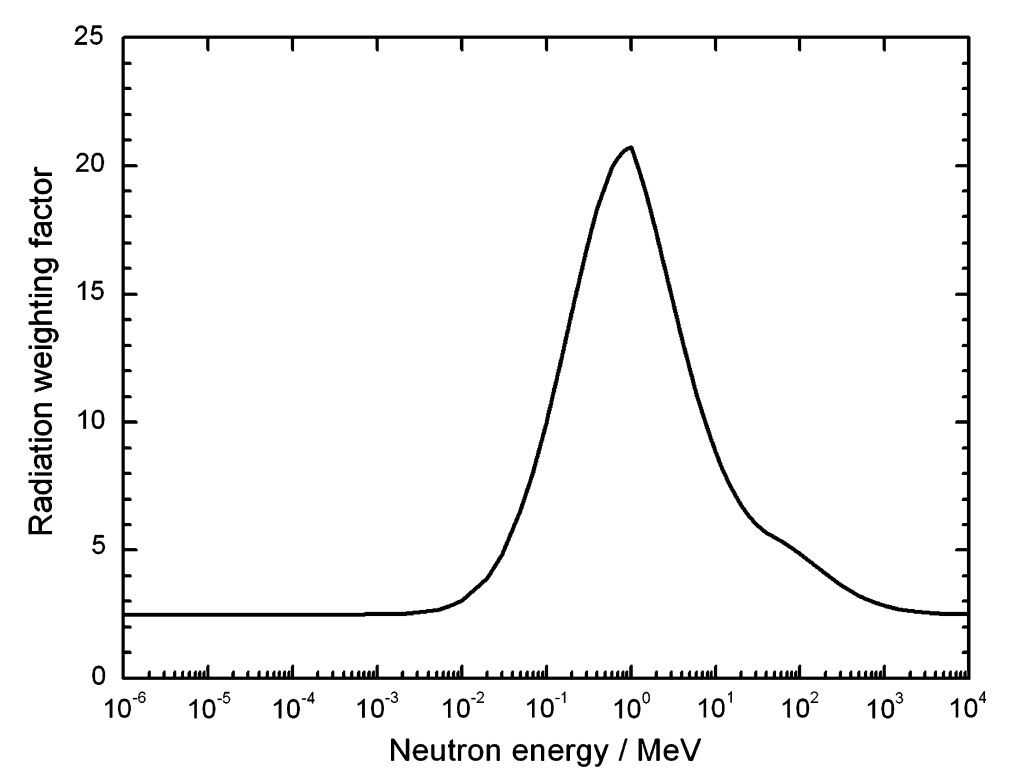
\includegraphics[height=3cm]{images/neutron.jpg} \\
\footnotesize {Continuous function of neutron energy}
\end{minipage} \\
\bottomrule
\end{tabular}

\end{table}

\subsubsection{Effective Dose}
Effective dose extends the concept of equivalent dose by incorporating tissue weighting factors, $w_T$. These factors quantify the relative contribution of specific organs and tissues to the overall radiation detriment, and are represented in Table \ref{tab:wt_factors}. The values are derived from epidemiological and radiobiological data and reflect averaged population risk, making $E$ a comparative metric rather than an indicator of individual risk. Effective dose is defined as the sum of the equivalent doses received by individual organs and tissues, each weighted by its respective factor~\cite{6,13,14}:

\begin{equation}
E = \sum_T H_T \cdot w_T,\ \text{unit: } [\mathrm{Sv}]
\label{eq:effective_dose}
\end{equation}

% Small vertical space after surrounding text
\vspace{1em}

% Manual table title, numbered and added to LoT
\refstepcounter{table}
\label{tab:wt_factors}
\noindent\textbf{Table~\thetable.} Tissue weighting factors for each organ/tissue. Adapted from Ref.~\cite{15}.%
\addcontentsline{lot}{table}{\protect\numberline{\thetable}Tissue weighting factors for each organ/tissue.}

% Small space between title and table
\vspace{0.1em}

\begin{table}[H]
  \centering
  \begin{tabular}{p{0.58\textwidth} c c}
    \toprule
    \textbf{Tissues and Organs} & \textbf{Weighting Factor,$w_T$} & \textbf{$\sum w_T$} \\
    \midrule
    Red bone marrow, Colon, Lung, Stomach, Breast, Remaining tissues* & 0.12 & 0.72 \\
    Gonads & 0.08 & 0.08 \\
    Bladder, Esophagus, Liver, Thyroid & 0.04 & 0.16 \\
    Bone surface, Brain, Salivary glands, Skin & 0.01 & 0.04 \\
    \midrule
    & \textit{Total} & \textbf{1.00} \\
    \bottomrule
  \end{tabular}

  \vspace{0.3em}
  {\footnotesize *Adrenals, Extrathoracic region,
Gall bladder, Heart, Kidneys, Lymphatic nodes, Muscle, Oral
mucosa, Pancreas, Prostate, Small intestine, Spleen, Thymus, Uterus/cervix}
\end{table}
\subsection{Operational Quantity}
In operational dosimetry, equivalent and effective dose cannot be measured directly~\cite{13}. Personal dosimetry is the applied science of using individual monitoring devices to estimate dose from occupational exposure. These devices are calibrated in terms of the personal dose equivalent, $H_p(d)$, defined as the dose equivalent in soft tissue at a depth $d$~mm beneath a specified point on the body and is expressed in Sv. At 10 mm, $H_p(10)$ is used to estimate effective dose from deeply penetrating radiation and is the principal quantity for assessing whole-body exposure. Dosimeters intended to measure Hp(10) are calibrated using reference radiation qualities defined in ISO 4037-1~\cite{113}. During calibration, the dosimeter is mounted on a polymethyl methacrylate (PMMA) phantom, and the field is characterized in terms of \emph{air KERMA}. For each radiation energy $E$ and angle of incidence $\alpha$, the International Commission on Radiation Units and Measurements (ICRU) provides conversion coefficients $h_{pK}(10; E, \alpha)$, which relate \emph{air KERMA} to $H_p(10)$~\cite{ICRU53}:
\begin{equation}
H_p(10) = h_{pK}(10; E, \alpha)\cdot K_{\mathrm{air}}, \quad [\mathrm{Sv}]
\label{eq:hp10}
\end{equation}

The same calibration approach applies to the assessment of equivalent dose, for which shallower depths are used. At 0.07 mm, $H_p(0.07)$ is used to assess dose to the skin from weakly penetrating radiation, and at 3 mm, $H_p(3)$  has been proposed specifically for the lens of the eye~\cite{13}.

\section{Occupational Exposure}
As previously mentioned, at the photon energies typical of fluoroscopy (recall Table~\ref{tab:ir_parameters}), the Compton effect predominates, degrading image quality and generating scattered radiation throughout the room \cite{6,23}. This stray radiation is the main source of occupational exposure for staff \cite{24}. From a dosimetric perspective, characterising the IR settings is inherently challenging due to the variability of parameters that influence radiation output and scatter distribution \cite{30}. In general, exposure to staff is proportional to the dose received by the patient \cite{21}. Tube voltage and current are adjusted based on patient size and anatomy during procedure planning, which in turn influence the amount of scatter produced \cite{30,31}. In addition, FOV and beam filtration also play a role, though their effects are not linear and highly dependent on scatter geometry \cite{32}. Beyond equipment settings, procedural complexity and operator technique contribute to variations in staff exposure. Advanced or prolonged interventions typically require longer fluoroscopy times, more image acquisitions, and non-standard projections \cite{30}. Operator experience has been shown to significantly reduce exposure through more efficient techniques, reduced reliance on fluoroscopy, and better positioning practices \cite{33}.

To illustrate scatter behaviour in a real clinical context, Fig.~\ref{fig:scatter} presents an isodose map, at chest height, generated during a fluoroscopically guided hip replacement procedure, and highlights the locations typically occupied by staff \cite{34}. The image reveals an asymmetric scatter pattern, with notably higher intensities recorded opposite to the position of the C-arm. The referenced study also reported lower dose levels on the side opposite the patient table, where equipment provides partial shielding. Although the inverse square law does not perfectly apply in the clinical environment \cite{35} due to scattering within the patient and surrounding structures, a general decrease in dose rate with increasing distance was still evident \cite{34}. This reaffirms the protective effect of physical separation from the source \cite{36}.
\begin{figure}[H]
  \centering
  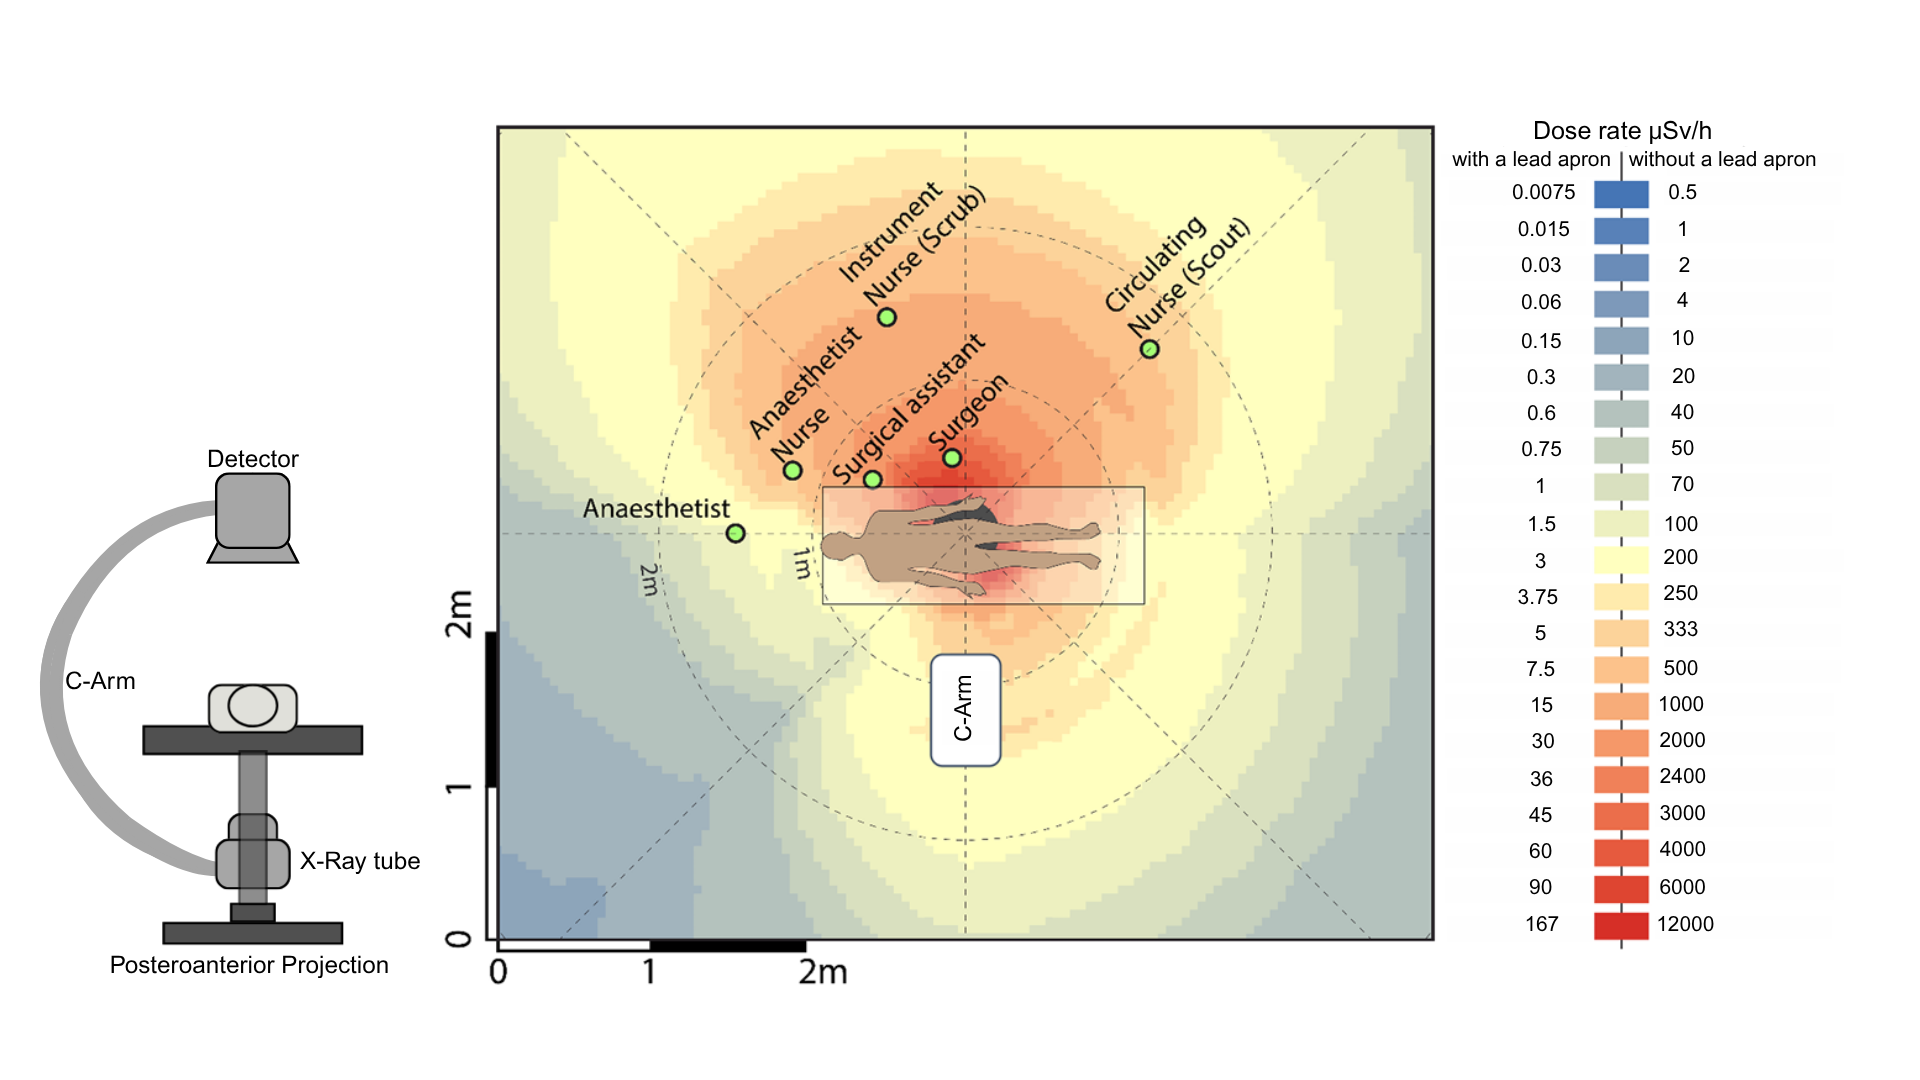
\includegraphics[width=\linewidth]{images/dose rates.png}
  \caption[Scatter radiation distribution in IR environment.]{Isodose map of scatter radiation during a fluoroscopically guided hip replacement procedure. Acquisition parameters included 77~kVp, 20.6~mA, 32.1~s of fluoroscopy time, and a pulse rate of 15~fps. Dose rates were measured using an active dosimeter at multiple positions around the phantom and linearly interpolated to generate the map. Values incorporating shielding (right scale) were estimated using theoretical models. Measurements are documented at chest level. The image was adapted from Ref.~\cite{34}. Although the C-arm configuration was not explicitly reported, a posteroanterior projection (left icon) was inferred based on findings from Ref.~\cite{35}.
  }

  \label{fig:scatter}
\end{figure}

Protection against cumulative exposure requires consistent application of shielding practices \cite{37}. Shielding is implemented at multiple levels, including structural room design, fixed barriers, and mobile shields, which contribute to protecting helping staff \cite{38} and sensitive areas such as the head and eyes, respectively~\cite{39}. However, personal protective equipment remains the most reliable and controllable form of protection. According to ICRP recommendations, all staff should wear lead aprons, along with thyroid shields, during fluoroscopic procedures \cite{37,39}. Most aprons have a lead thickness range of 0.35 to 0.5~mm, with 0.5~mm reducing scattered radiation by over 90\% \cite{37}. To be effective, aprons must fit properly, and facilities should be encouraged to invest in a variety of sizes to ensure proper coverage and comfort \cite{38,40}. Thyroid shields are manufactured with a lead equivalence of 0.5~mm and have been reported to reduce exposure to the gland by approximately 50\% \cite{41}. %Their use is particularly advised for staff who receive monthly collar readings above 4~mSv and are under 40 years of age, due to the increased risk of thyroid cancer \cite{42}.
Lead glasses are also available but remain underutilised. As the second most effective protective measure after ceiling-suspended shields, these glasses are available in various frame designs and thicknesses ranging from 0.35 to 0.75~mm. %Their protective benefit, however, depends greatly on the positioning of the operator’s head in relation to the patient during procedures \cite{40}.

 The effectiveness of these protective measures is ultimately verified against the annual occupational dose limits recommended by the ICRP, summarised in Table \ref{tab:occupational_dose_limits}. These limits are not an absolute safety threshold but rather boundaries beyond which cumulative exposures are no longer considered justified~\cite{13}. For instance, the $E$ limit for radiation workers is set at 20~mSv per year, averaged over five years, with an upper limit of 50~mSv in any single year \cite{15}.




\vspace{1em}

\refstepcounter{table}
\label{tab:occupational_dose_limits}
\noindent\textbf{Table~\thetable.} ICRP occupational dose limits. Adapted from Refs.~\cite{15,44}.%
\addcontentsline{lot}{table}{\protect\numberline{\thetable}ICRP occupational dose limits.}

\vspace{0.1em}


\begin{table}[H]
\centering
\renewcommand{\arraystretch}{1.4}
\setlength{\tabcolsep}{8pt}
\begin{tabular}{
  >{\centering\arraybackslash}m{0.22\textwidth}
  >{\centering\arraybackslash}m{0.33\textwidth}
  >{\centering\arraybackslash}m{0.33\textwidth}}
\toprule
\multicolumn{2}{m{0.55\textwidth}}{\centering\textbf{Protection Quantity}} & \textbf{Annual Permissible Dose} \\
\midrule
\multicolumn{2}{m{0.55\textwidth}}{
  \centering\textbf{Effective Dose}
} &
\begin{minipage}[c][3.5\baselineskip][c]{\linewidth}
\centering
20 mSv per year averaged over 5 years \\
(no single year exceeding 50 mSv)
\end{minipage} \\
\midrule
\multirow{3}{=}{\textbf{Equivalent Dose}}
& Lens of the Eyes & 20 mSv \\
& Thyroid Gland & 300 mSv \\
& Individual Organs (excluding the eye), Skin and Extremity & 500 mSv \\
\bottomrule
\end{tabular}
%\caption{Annual permissible dose limits for various protection quantities.}
\end{table}

As previously introduced, currently, compliance with occupational dose limits in IR is verified through routine monitoring using passive dosimeters worn by staff over predefined time intervals. The most common devices are thermoluminescent dosimeters and optically stimulated luminescence dosimeters. Both operate by trapping energy when exposed to ionising radiation, which is later released as light when stimulated under controlled conditions. The intensity of the emitted light is proportional to the amount of absorbed radiation \cite{11}. These devices measure the previously discussed quantity $H_p(10)$. While $H_p(10)$ can serve as an approximation of effective dose under conditions of uniform whole-body exposure, this does not reflect the typical environment in IR, as described \cite{64}. When a single dosimeter is used, placement beneath the lead apron tends to underestimate $E$ due to shielding, while positioning it above may overestimate it~\cite{30}. To improve accuracy, the ICRP recommends a dual dosimetry approach. In this method, one dosimeter is worn underneath the protective apron between the waist and chest to record the attenuated exposure to shielded tissues ($H^u$). The second device is placed at collar level outside the apron to monitor exposure to unshielded regions ($H^o$). An effective dose estimate is then calculated by applying a linear combination of these two measurements \cite{65}:

\begin{equation}
E = \alpha H^u + \beta H^o,\ \text{unit: } [\mathrm{Sv}]
\label{eq:dual_dosimetry}
\end{equation}

However, there is currently no global consensus on the value of both weighting factors, $\alpha$ and $\beta$ \cite{65}. Over 14 different algorithms have been reported in the literature, most of which overestimate $E$. Despite this variability, double dosimetry remains more accurate than single-dosimeter methods \cite{66}.

The major limitation of passive dosimeters lies in their inability to provide dose information in real-time. These devices are typically read at monthly intervals \cite{67}, which prevents identification of excessive exposures or deviations from standard operating conditions in time. As a result, opportunities for real-time corrective action are lost, and staff may remain unaware of elevated exposure levels until the data can be reviewed retrospectively \cite{46,68}. In this context, active personal dosimeters (APDs) have emerged as a complementary solution. APDs are not intended to replace passive dosimeters, which remain the standard for legal dose documentation. By providing real-time feedback on dose rate, APDs support adherence to the ALARA principle by enabling immediate adjustments to operator behaviour or shielding practices \cite{2,3}.

\section{Real-Time Dosimetry}
The concept of real-time radiation monitoring in occupational settings was first established through the use of APDs, which have been widely adopted in the nuclear industry as a standard safety practice \cite{69}. However, it was only within the last 15 years that their use in IR began to be critically evaluated \cite{2,38,69,70}. As previously discussed, the IR environment is characterised by pulsed radiation, lower photon energies, and predominantly scattered fields, which differ significantly from the conditions under which the APDs available at the time were originally developed \cite{70}. Although several studies \cite{20,69,70} explored the possibility of adapting existing devices for IR, it was Sánchez \emph{et al}. \cite{2}, working as part of an early development initiative at Philips, who introduced the first APD specifically engineered for interventional use. Unlike existing APDs that provided exclusively auditory feedback, this prototype included a visual interface displaying real-time dose data to staff in the procedure room. It became the first generation of the DoseAware system, which started being distributed commercially in 2010 \cite{71}. Later, Philips and Unfors RaySafe signed a joint development agreement in 2012 and, in 2017, the third-generation system, RaySafe i3, was introduced at the European Congress of Radiology \cite{76}.

The device features a silicon solid-state diode \cite{72}, integrated into an invididual wearable bagde with wireless capabilities, transmitting scattered dose information to a data collection unit at a one second rate. Detected dose values are displayed on an in-room monitor as both numerical data and a bar graph. Each badge is represented individually, with exposure levels indicated using a colour-coded scheme (green, yellow, and red) corresponding to increasing dose rates~\cite{2}.
The operational photon energy range of the system is N40--N150 for X- and $\gamma$-radiation. The relative measurement uncertainty is approximately 10\% for dose rates in the range of 40--150~$\mu$Sv/h and 20\% for dose rates between 150--300~$\mu$Sv/h. The system has been shown to correlate well with legal-for-record passive dosimeters, typically overestimating $H_{\mathrm{p}}(10)$ by 5--15\%.

The collaboration between Philips and RaySafe enabled the integration of badge-derived data into dedicated software platforms, such as Dose Viewer and Dose Manager \cite{81}. These platforms support retrospective analysis by allowing users to access, export, and manage individual dose histories, as well as aggregate exposure data across teams or departments. RaySafe i3 is currently priced at around 27,000\euro~\cite{79}, which raises concerns about cost. Individual APD units are expensive, making it difficult for most imaging departments to provide them for all staff. In addition, current systems do not support extremity monitoring, such as for the eyes or hands \cite{80}.

\subsection{Reported Benefits}
The development and clinical integration of the APDs described above enabled structured evaluation of their practical impact in IR. Since their introduction, a number of studies have compared conditions with and without real-time feedback~\cite{4,68,72,82,83,85,86,87,88,114,115,116}. A common finding is a general decrease in staff dose when feedback is available. This effect appears across various professional roles, though the degree of reduction can vary. In a study led by Baumann \emph{et al}~\cite{86} dose reduction was observed in almost every staff group~\cite{86}. Further analysis reveals a pattern seen across multiple studies, where the most significant reductions are recorded in the main radiologist, who is positioned closest to the patient. In some studies, this group was the only one to show a statistically significant change in radiation exposure~\cite{72,86,87,88}. This may be explained by findings from Baumgartner \emph{et al}\ \cite{72}, which showed that procedural contexts associated with higher radiation exposure tend to demonstrate the most pronounced reductions following the introduction of APDs \cite{72}. This is consistent with reports that the effectiveness of APDs depends on baseline conditions. Operators who initially demonstrated poor radiation safety habits were able to significantly reduce their dose after the introduction of APDs through simple corrective actions. In contrast, those already practising good protection strategies had less room to improve and showed minimal change \cite{82,87,115}. These baseline variations are also associated with the operator’s level of experience, as discussed in section~1.4, and were recently studied by Koch \emph{et al}~\cite{83}. A pronounced decrease in dose was registered among the least experiences group, while operators with over ten years of experience show, in this case, even a slight increase in dose. Experienced operators may rely on ingrained habits and confidence in their technique, whereas less experienced users appear to adjust more readily when confronted with live feedback \cite{83}. It has been reported that younger operators tend to show less concern for radiation safety \cite{89}. These results suggest that APDs may be especially valuable as educational tools for junior staff, helping them build good radiation safety practices \cite{83}.

Consistent with these findings, James \emph{et al}~\cite{115}, reported a reduction in red events over time. They argued that, while these events serve as prompts for immediate dose adjustment, they also function as a reflective tool for operators. This enables professionals to identify specific maneuvers, projection angles, and procedural choices associated with increased radiation exposure. Consequently, such practices can be replaced by lower-exposure alternatives and operators can adopt safer procedural habits more permanently. Ultimately, it also contributes to a reduction in radiation dose to the patient~\cite{115,116}.

Other staff members, including nurses and technicians, also benefited from dose reductions \cite{82,83,85,86,88,115}. In these cases, it was primarily attributed to individual awareness and simple adjustments, such as changes in positioning. Some studies further emphasised the collaborative value of these systems, noting that when all staff members wear APDs with visible displays, teams can collectively monitor exposure. This practice creates an environment of mutual accountability, where individuals not only adjust their own behaviour but also remain aware of their colleagues’ exposure, promoting safer team dynamics \cite{86,87,115}.
